\documentclass{article}

\usepackage[vmarginratio=1:1,a4paper,body={6.5in, 9.5in}]{geometry}

\usepackage[T2A]{fontenc}
\usepackage[utf8]{inputenc}
\usepackage[russian]{babel}

\usepackage{amsmath}
\usepackage{amssymb}
\usepackage{amsfonts}
\usepackage{amsthm}
\usepackage{color}

\usepackage{hyperref}
\usepackage{graphicx}


\title{Reaction wheel 1D pendulum}
\author{}
\date{}

\begin{document}

\maketitle
% The Reaction Wheel Pendulum (Block, Atrom, Spong)
%ftp://nozdr.ru/biblio/kolxo3/P/PC/PCtm/Block%20D.,%20Astroem%20K.,%20Spong%20M.%20The%20Reaction%20Wheel%20Pendulum%20(MC,%202007)(ISBN%201598291947)(O)(112s)_PCtm_.pdf

\begin{itemize}
    \item $m_p$ - масса маятника
    \item $m_r$ - масса ротора
    \item $l_p$ - расстояние от шарнира до центра масс маятника
    \item $l_r$ - расстояние от шарнира до центра масс ротора
    \item $J_p$ - момент инерции маятника при вращении вокруг центра масс
    \item $J_r$ - момент инерции ротора
    \item $\theta$ - угол маятника относительно вертикали
    \item $\theta_r$ - угол ротора \textbf{относительно маятника}
    \item $\tau$ - момент, прикладываемый к ротору
    \item $C_p$ - коэффициент вязкого трения в шарнире маятника
    \item $C_r$ - коэффициент вязкого трения ротора
\end{itemize}

Кинетическая энергия маятника:
$$
T_p = \frac{1}{2} (m_pl_p^2 + J_p)\dot\theta^2
$$

Кинетическая энергия маховика:
$$
T_r = \frac{1}{2} m_r l_r^2 \dot\theta^2 + \frac{1}{2}J_r (\dot\theta_r+\dot\theta)^2
$$

Общая потенциальная энергия:
$$
P = (m_pl_p + m_r l_r)g \cos\theta
$$

Лагранжиан:
$$
\mathcal{L} = T_p + T_r - P
$$

Введём новые обозначения констант, которые нам уменьшат общее количество закорючек в уравнениях:
\begin{align*}
ml&:=m_p l_p + m_r l_r\\
J &:= J_p + m_p l_p^2 + m_r l_r^2
\end{align*}

Тогда лагранжиан запишется следующим образом:
$$
\mathcal L = \frac{1}{2}J\dot\theta^2 + \frac{1}{2}J_r(\dot\theta_r+\dot\theta)^2 - mlg\cos\theta
$$

Для удобства выпишем все частные производные:
\begin{align*}
\frac{\partial\mathcal L}{\partial\dot\theta_r} &= J_r(\dot\theta_r + \dot\theta)       & \frac{\partial\mathcal L}{\partial\theta_r} &= 0            \\
\frac{\partial\mathcal L}{\partial\dot\theta}   &= (J+J_r)\dot\theta + J_r\dot\theta_r  & \frac{\partial\mathcal L}{\partial\theta}   &= mlg\sin\theta\\
\end{align*}

Напоминалка про уравнения Лагранжа:
$$
\frac{d}{dt}\left(\frac{\partial\mathcal L}{\partial\dot q_i}\right) - \frac{\partial\mathcal L}{\partial q_i} = \tau_i
$$

Тогда уравнения движения примут следующий вид:
\begin{align*}
J_r\ddot\theta_r + J_r\ddot\theta&= - C_r \dot\theta_r + \tau\\
(J+J_r)\ddot \theta + J_r\ddot\theta_r - mlg\sin\theta &= - C_p \dot\theta 
\end{align*}

Перепишем, оставив вторые производные слева:
$$
\left\{
\begin{array}{l}
\ddot\theta_r = \frac{J+J_r}{J J_r}(\tau - C_r\dot\theta_r) - \frac{mlg}{J}\sin\theta + \frac{C_p}{J}\dot\theta\\
\ddot\theta   = -\frac{\tau}{J} + \frac{ml g}{J}\sin\theta  - \frac{C_p}{J} \dot\theta + \frac{C_r}{J} \dot\theta_r
\end{array}
\right.
$$



Наверняка трение в маятнике будет существенно ниже трения в роторе, и вполне возможно, что при этом пренебречь можно будет обоими. 


{\color{red} Эти уравнения движения полностью совпадают с уравнениями из \href{https://www.ethz.ch/content/dam/ethz/special-interest/mavt/dynamic-systems-n-control/idsc-dam/Research_DAndrea/Cubli/Cubli_IROS2012.pdf}{The Cubli: A Cube that can Jump Up and Balance}, а также с уравнениями из \href{https://dl.acm.org/citation.cfm?id=3019246}{The Reaction Wheel Pendulum} (с точностью до выбора переменных, Åström отсчитывает угол ротора от вертикали). Но Åström в уравнения Лагранжа вставляет моменты $\tau$ и $-\tau$, а я тут вставляются $\tau$ и 0. Подход Острёма интуитивно понятен: если на ротор действует момент $\tau$, то на маятник действует момент $-\tau$. Впрочем, это зависит от выбора репера ($\theta_r$ отсчитывается от вертикали или от маятника). Нечего выбирать неортогональные базисы пространства конфигураций.}


\section{Как выбрать размер маховика?}

Здесь я напишу уравнения движения для обычного коллекторного двигателя, но для бесколлекторных уравнения примерно такие же.  Подадим на клеммы мотора максимально возможное напряжение, для заданного маховика задача состоит в том, чтобы найти максимально возможный угол начального отклонения маятника, при котором разгоняющийся маховик сможет перекинуть маятник через ноль. Затем будем варьировать размер маховика и смотреть, как будет изменяться максимально возможный угол отклонения.

Заглянем в даташит мотора:
\begin{itemize}
    \item $L$ - индуктивность обмотки
    \item $R$ - сопротивление обмотки
    \item $k$ - torque constant (= back-EMF constant)
\end{itemize}

Добавим в уравнения движения уравнение мотора:
$$
\left\{
\begin{array}{l}
\ddot\theta_r = \frac{J+J_r}{J J_r}(kI - C_r\dot\theta_r)  -mlg/J\sin\theta + C_p/J\dot\theta\\
\ddot \theta  = -k/J I + mlg/J\sin\theta - C_p/J \dot\theta + C_r/J \dot\theta_r\\
\dot I  = U/L - R/LI - k/L \dot\theta_r\\
\end{array}
\right.
$$

Решаем численно, перебираем значения обычными вложенными циклами. Зависимость максимального угла от радиуса маховика (алюминиевый цилиндр высоты 20мм) выглядит следующим образом (ниже 20мм радиуса не стабилизируется вообще):

\centerline{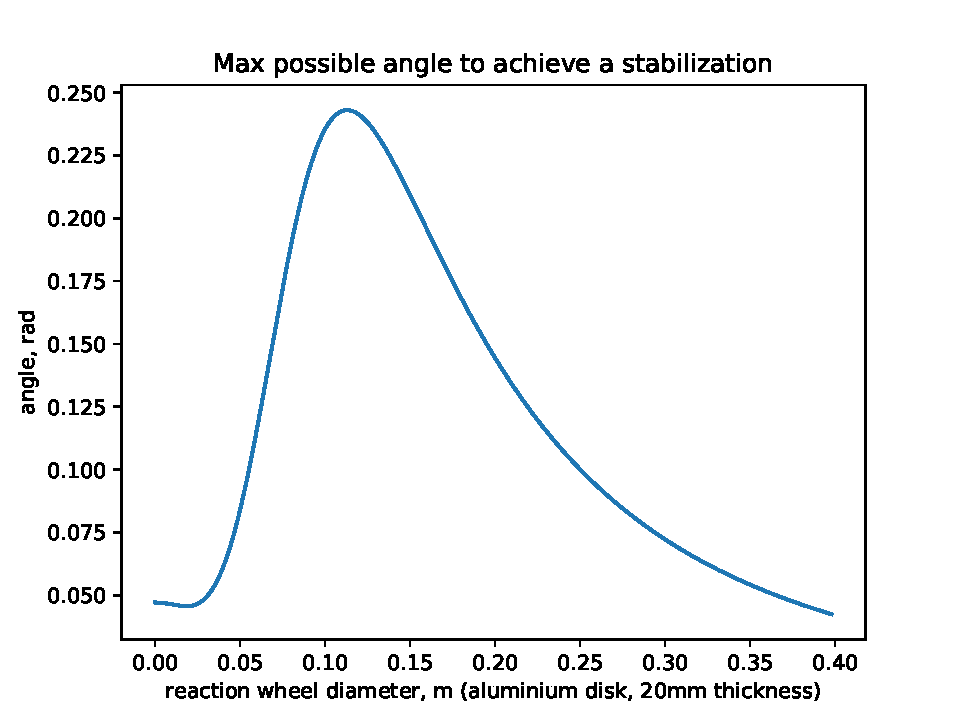
\includegraphics[width=.8\linewidth]{img/pendulum_dynamics}}

Получается, что чем меньше маховик, тем легче стабилизировать (меньше массы поднимать), при этом быстрый подъём противо-ЭДС никого не волнует, системе выгоднее дать короткий, но сильный импульс. В таких условиях мне кажется наиболее разумным выбор маховика диаметром эдак сантиметров 10 (это уже полкило, если что).


\newpage
\section{Давайте разбираться с моментами}
Силы тяжести нет, трения нет, все моменты инерции равны единице.
$$
q_v = q_p + \theta
$$

\subsection{Неподвижный репер}

Возьмём в качестве обобщённых координат $\theta$ и $q_v$. Тогда лагранжиан запишется так:
$$
\mathcal{L} = \frac{1}{2} \dot \theta^2 + \frac{1}{2}\dot q^2_v
$$

Для удобства выпишем все частные производные:
\begin{align*}
\frac{\partial\mathcal L}{\partial\dot q_v} &= \dot q_v   && \frac{\partial\mathcal L}{\partial q_v} = 0\\
\frac{\partial\mathcal L}{\partial\dot\theta} &= \dot\theta && \frac{\partial\mathcal L}{\partial\theta} = 0\\
\end{align*}

Выпишем уравнения Лагранжа:

\begin{align*}
\frac{d}{dt}\left(\frac{\partial\mathcal L}{\partial\dot q_v}\right) - \frac{\partial\mathcal L}{\partial q_v} = \ddot q_v = \tau\\
\frac{d}{dt}\left(\frac{\partial\mathcal L}{\partial\dot \theta}\right) - \frac{\partial\mathcal L}{\partial \theta} = \ddot\theta = -\tau\\
\end{align*}

\subsection{Вращающийся репер}

Возьмём в качестве обобщённых координат $\theta$ и $q_p$. Тогда лагранжиан запишется так:
$$
\mathcal{L} = \frac{1}{2} \dot \theta^2 + \frac{1}{2}(\dot q_p+\dot\theta)^2
$$

Для удобства выпишем все частные производные:
\begin{align*}
\frac{\partial\mathcal L}{\partial\dot q_p} &= \dot q_p + \dot\theta && \frac{\partial\mathcal L}{\partial q_p} = 0\\
\frac{\partial\mathcal L}{\partial\dot\theta} &= 2\dot\theta +\dot q_p &&  \frac{\partial\mathcal L}{\partial\theta} = 0\\
\end{align*}

Выпишем уравнения Лагранжа. Предположим, что я не знаю действующих моментов, обозначу их через $x$ и $y$, буду их искать так, чтобы уравнения совпали с уравнениями из предыдущего параграфа.

\begin{align*}
\frac{d}{dt}\left(\frac{\partial\mathcal L}{\partial\dot q_p}\right) - \frac{\partial\mathcal L}{\partial q_p}= \ddot q_p + \ddot\theta = x\\
\frac{d}{dt}\left(\frac{\partial\mathcal L}{\partial\dot \theta}\right) - \frac{\partial\mathcal L}{\partial \theta}= 2\ddot\theta +  \ddot q_p   = y\\
\end{align*}

Перепишем наши уравнения движения следующим образом:

\begin{align*}
\ddot q_p = 2x - y\\
\ddot\theta = y - x
\end{align*}

Очевидно, что если $\ddot q_v = \tau$, то $\ddot q_p = 2\tau$, поскольку $q_v = q_p + \theta$, а $\ddot\theta = -\tau$. Запишем уравнения для $x$ и $y$:

\begin{align*}
\ddot q_p = 2x - y = 2\tau\\
\ddot\theta = y - x = -\tau
\end{align*}

Решением является $x=\tau, y=0$. ЧТД.


\end{document}
